% Created 2014-02-07 Fri 17:32
\documentclass[sans,aspectratio=169,presentation,bigger,fleqn]{beamer}
\usepackage[utf8]{inputenc}
\usepackage[T1]{fontenc}
\usepackage{fixltx2e}
\usepackage{graphicx}
\usepackage{longtable}
\usepackage{float}
\usepackage{wrapfig}
\usepackage{rotating}
\usepackage[normalem]{ulem}
\usepackage{amsmath}
\usepackage{textcomp}
\usepackage{marvosym}
\usepackage{wasysym}
\usepackage{amssymb}
\usepackage{hyperref}
\tolerance=1000
\usepackage{setspace}
\setstretch{1.3}
\usepackage{booktabs}
\hypersetup{colorlinks=true,linkcolor=blue,urlcolor=blue}
%\usetheme{naked}
\usepackage{lmodern}
\usetheme[alternativetitlepage=true,titleline=true]{Torino}
\usecolortheme{freewilly}
\usetheme{default}
\author{John Henderson}
\date{08 February 2014}
\title{Working with geo-spatial data in R}
\hypersetup{
  pdfkeywords={},
  pdfsubject={},
  pdfcreator={Emacs 24.3.1 (Org mode 8.2.5h)}}
\begin{document}

\maketitle


\begin{frame}[fragile,label=sec-1]{Intro}
 \begin{itemize}
\item Rapid fire overview of geo-spatial miscellany in \texttt{R}
\item If you're not familiar with \texttt{R}, don't worry about the code
\item The code/data necessary to reproduce anything in this talk is all on \href{https://github.com/jwhendy/devFest-geo}{github}!
\end{itemize}

\vspace{1cm} \pause

\alert{My goal}

Show you enough relatively cool things in 15min to entice you to give \texttt{R} a shot!
\end{frame}
\begin{frame}[fragile,label=sec-2]{Using \texttt{ggmap} to get lat/lon coordinates}
 \begin{itemize}
\item Just type what you wold type into Google Maps
\end{itemize}


\scriptsize

\begin{verbatim}
  # install.packages("ggmap")
  library(ggmap)
  geocode("St. Paul, MN")
\end{verbatim}
\begin{verbatim}
        lon     lat
1 -93.08996 44.9537
\end{verbatim}

\begin{verbatim}
  geocode("2115 Summit Ave., St. Paul, MN")
\end{verbatim}
\begin{verbatim}
        lon      lat
1 -93.18971 44.94412
\end{verbatim}

\begin{verbatim}
  geocode("University of St. Thomas, MN")
\end{verbatim}
\begin{verbatim}
        lon      lat
1 -93.18975 44.94192
\end{verbatim}

\normalsize
\end{frame}

\begin{frame}[label=sec-3]{Grabbing maps}
Methods
\begin{itemize}
\item Lat/lon + zoom level
\item Bounding box
\end{itemize}

Sources
\begin{itemize}
\item Google
\item Stamen
\item Cloudmade
\item OpenStreetMap
\end{itemize}
\end{frame}
\begin{frame}[fragile,label=sec-4]{Using lat/lon + zoom}
 \begin{verbatim}
loc <- geocode("2115 Summit Ave, St. Paul, MN")
ust <- get_map(location = c(lon = loc$lon, lat = loc$lat),
                zoom = 15, source = "google",
                maptype = "hybrid", crop = T)

ggmap(ust)
\end{verbatim}
\end{frame}
\begin{frame}[label=sec-5]{Using lat/lon + zoom}
\begin{center}
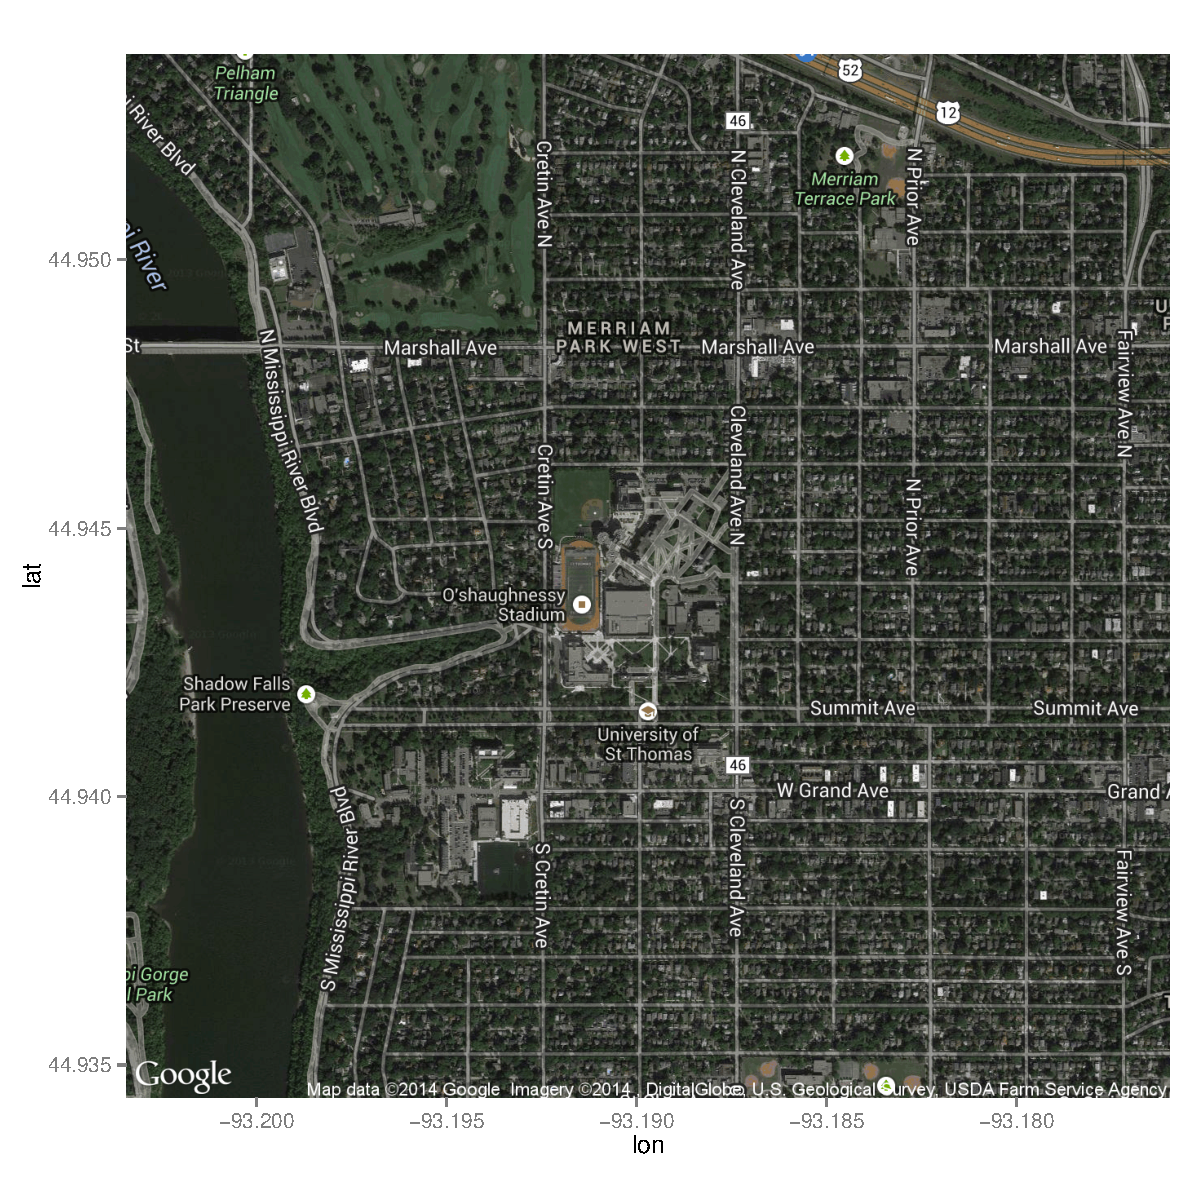
\includegraphics[height=6.5cm]{./plots/ust-coords-zoom.pdf}
\end{center}
\end{frame}
\begin{frame}[fragile,label=sec-6]{Using lat/lon + bounding box}
 \begin{verbatim}
loc <- geocode("2115 Summit Ave, St. Paul, MN")

box <- c(left = loc$lon - 0.04, bottom = loc$lat - 0.02,
         right = loc$lon + 0.04, top = loc$lat + 0.02)

ust_box <- get_map(location = box, source = "stamen",
                   maptype = "watercolor", crop = T)

ggmap(ust_box)
\end{verbatim}
\end{frame}
\begin{frame}[label=sec-7]{Using lat/lon + bounding box}
\begin{center}
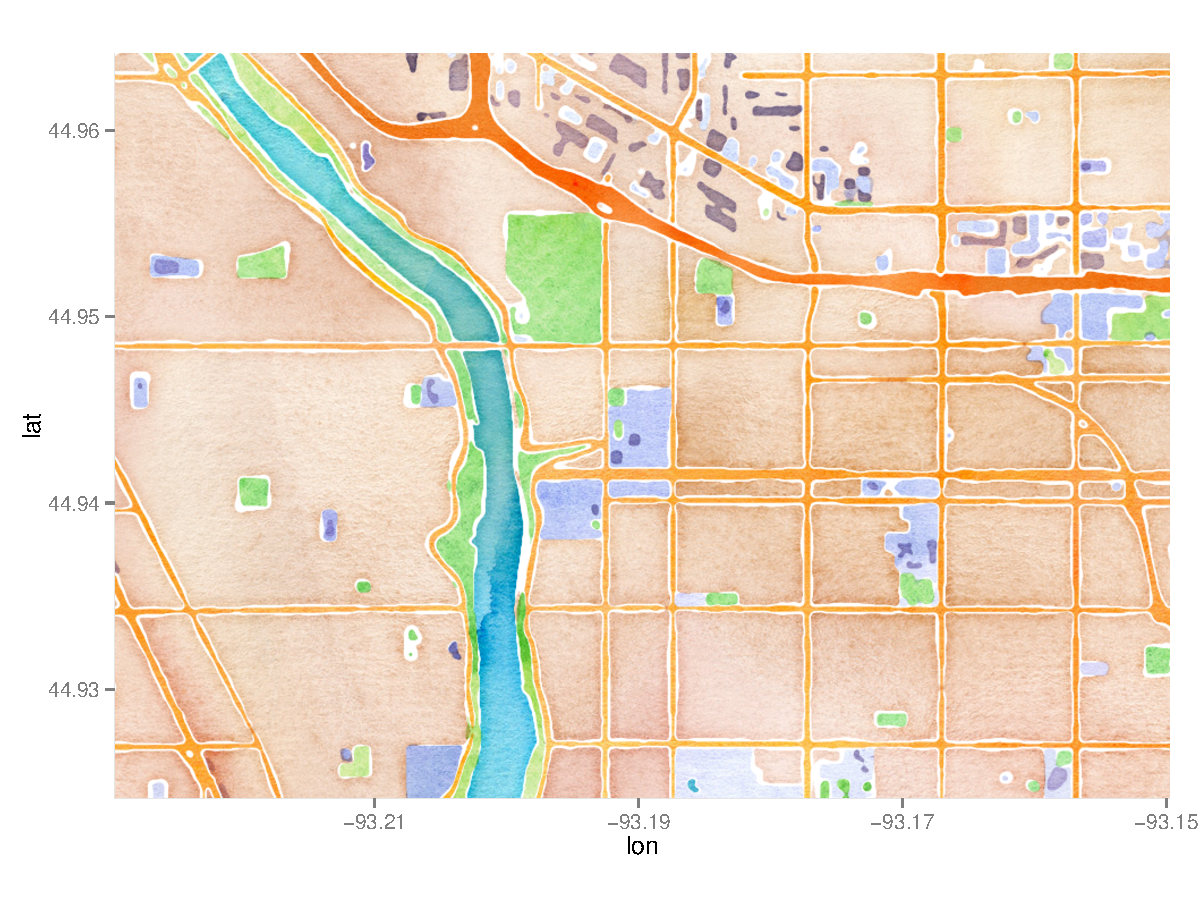
\includegraphics[height=6.5cm]{./plots/ust-coords-box.pdf}
\end{center}
\end{frame}
\begin{frame}[fragile,label=sec-8]{Overplotting maps}
 \begin{itemize}
\item \texttt{ggmap()} adds onto existing \texttt{ggplot2} functionality
\item Thus, layering standard \texttt{ggplot2} graphics on top of maps is easy!
\end{itemize}

\scriptsize
\begin{verbatim}
locs <- data.frame(names = c("st. paul", "minneapolis"))                  # grab locations
locs <- cbind(locs, geocode(as.character(locs$names)))

mid <- get_map(location = c(lon = mean(locs$lon), lat = mean(locs$lat)),  # get a map
               zoom = 10, source = "stamen", maptype = "toner", crop = T)

p <- ggmap(mid)                                                           # plot map
p <- p + geom_point(aes(x = lon, y = lat, colour = factor(names)),        # overplot w/ points
                    dat = locs, size = 6)
p <- p + scale_colour_discrete("Location")
\end{verbatim}

\normalsize
\end{frame}
\begin{frame}[label=sec-9]{Overplotting ggmaps}
\begin{center}
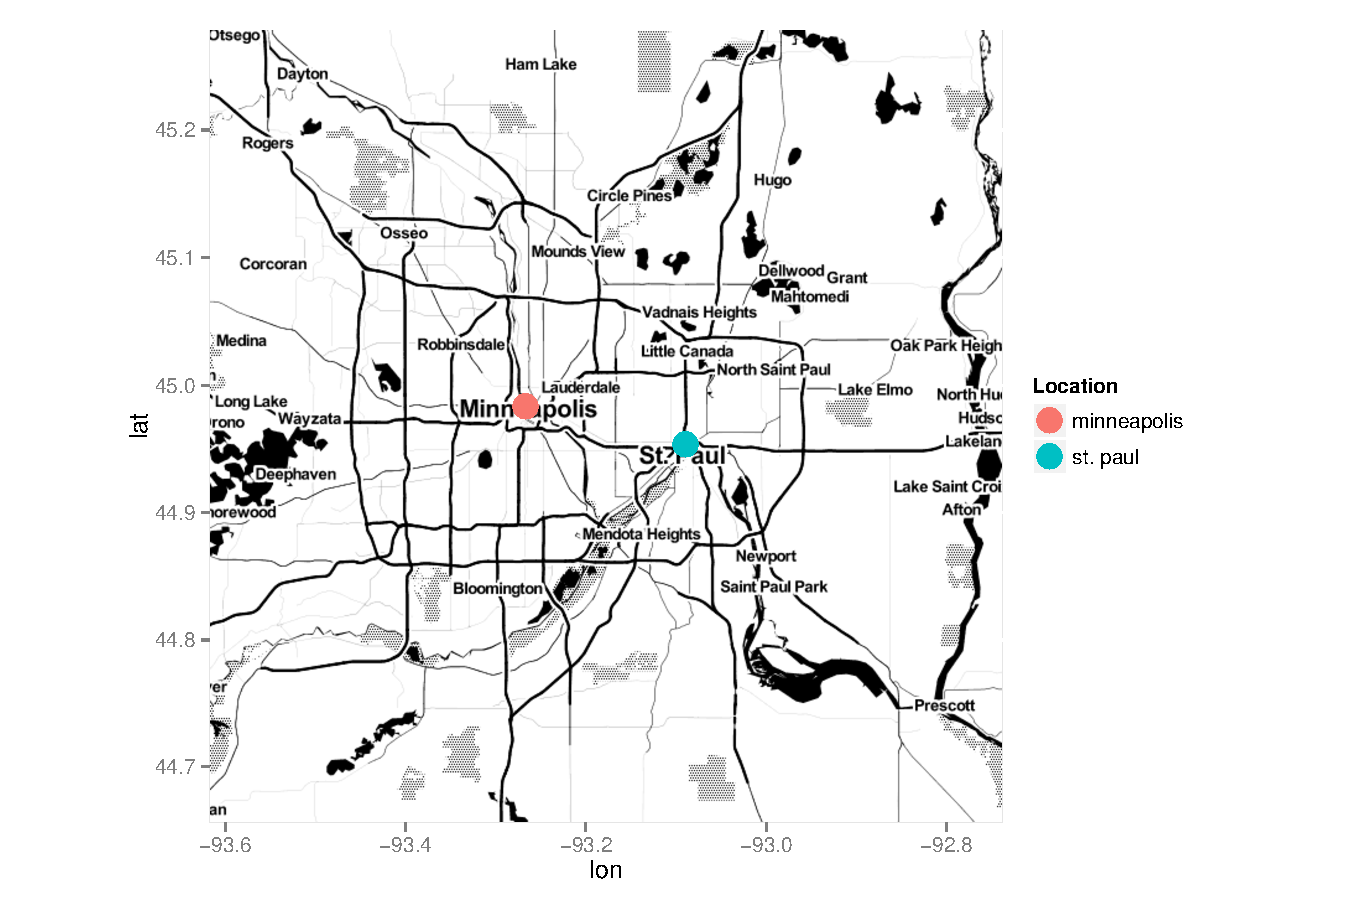
\includegraphics[height=6.5cm]{./plots/ggmap-points.pdf}
\end{center}
\end{frame}
\begin{frame}[fragile,label=sec-10]{Working with world/country maps}
 \begin{itemize}
\item \texttt{get\_map()} limited by allowable zoom levels (e.g. \texttt{0 < zoom < 21})
\item For larger scale data, the \texttt{maps} package is necessary
\item Various maps available; see the \href{http://cran.r-project.org/web/packages/maps/maps.pdf}{documentation}
\end{itemize}

\scriptsize
\begin{verbatim}
library(maps)
world <- map_data("world")
head(map, 5)
\end{verbatim}

\begin{verbatim}
       long      lat group order region subregion
1 -133.3664 58.42416     1     1 Canada      <NA>
2 -132.2681 57.16308     1     2 Canada      <NA>
3 -132.0498 56.98610     1     3 Canada      <NA>
4 -131.8797 56.74001     1     4 Canada      <NA>
5 -130.2492 56.09945     1     5 Canada      <NA>
\end{verbatim}
\end{frame}
\begin{frame}[fragile,label=sec-11]{World map example}
 \scriptsize
\begin{verbatim}
# pay attention to column names (long vs. lon!)
p <- ggplot(world, aes(x = long, y = lat, group = group))
p <- p + geom_polygon(colour = "white")
p
\end{verbatim}

\begin{center}
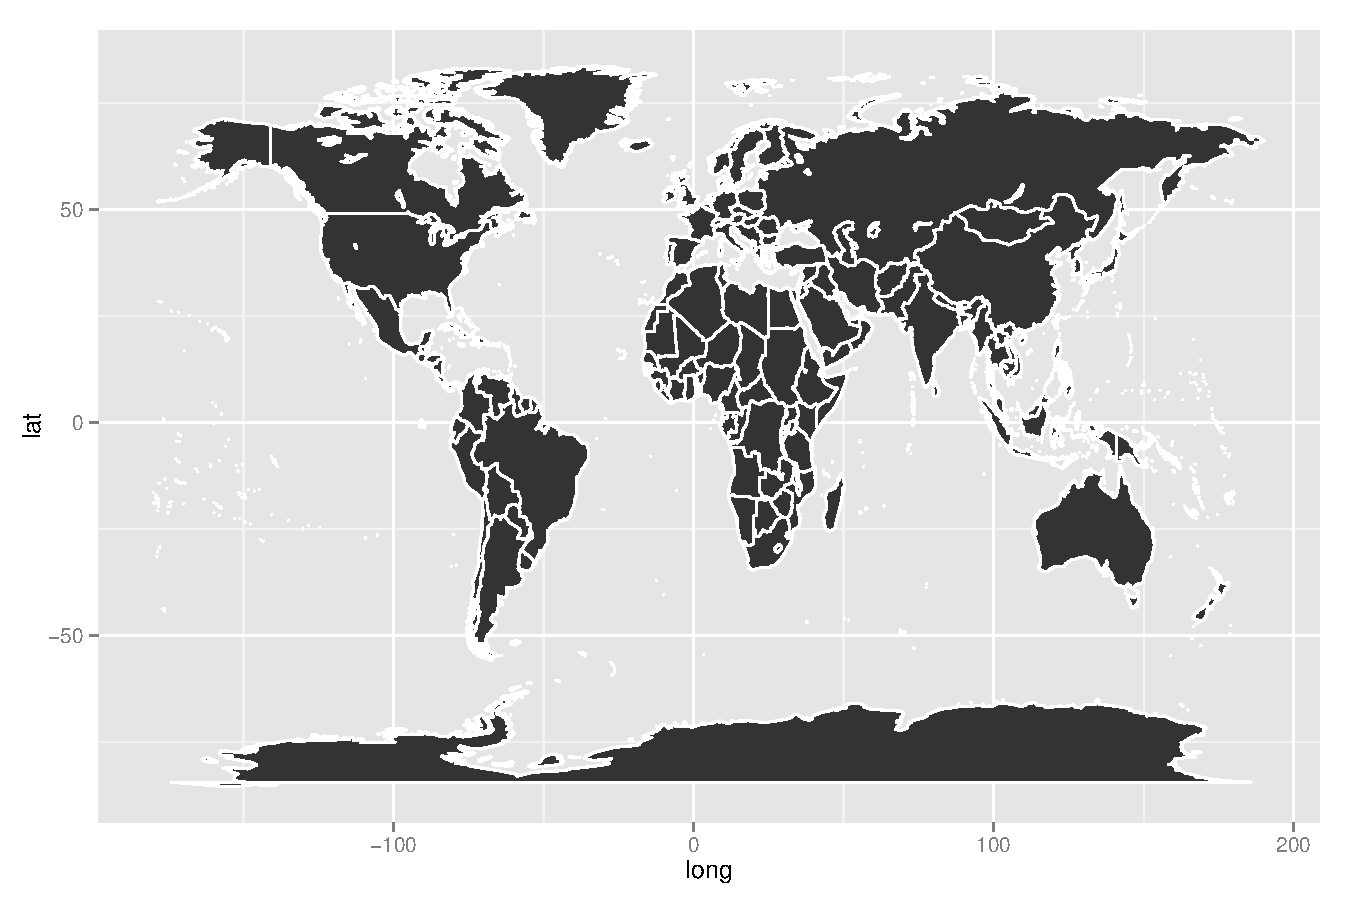
\includegraphics[height=4.5cm]{./plots/world.pdf}
\end{center}

\normalsize
\end{frame}
\begin{frame}[fragile,label=sec-12]{United States example}
 \scriptsize
\begin{verbatim}
usa <- map_data("state")
p <- ggplot(usa, aes(x = long, y = lat, group = group))
p <- p + geom_polygon(colour = "white")
p
\end{verbatim}

\begin{center}
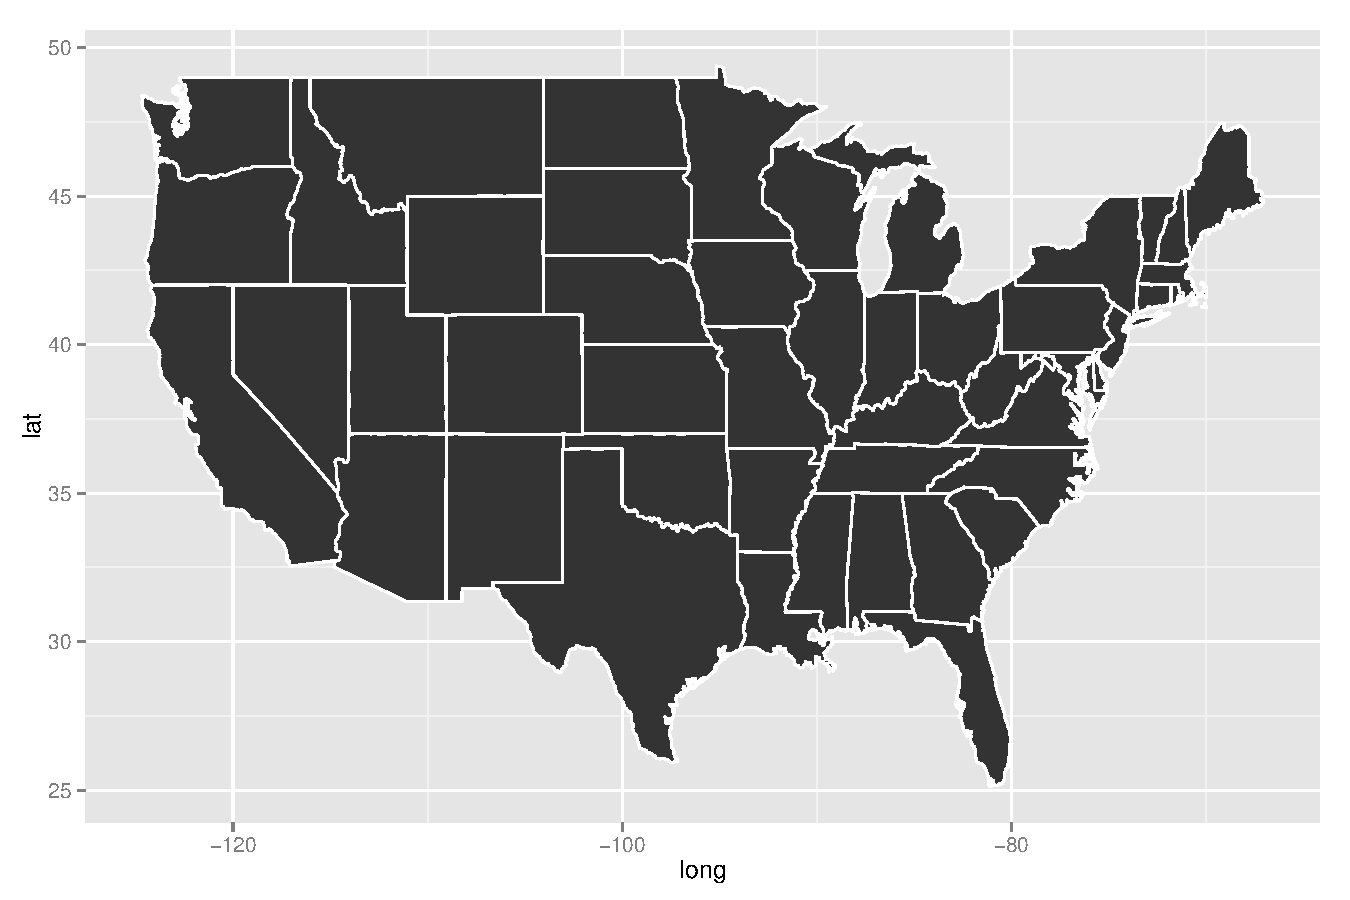
\includegraphics[height=4.5cm]{./plots/usa.pdf}
\end{center}

\normalsize
\end{frame}
\begin{frame}[fragile,label=sec-13]{Subsetting areas}
 \scriptsize
\begin{verbatim}
states <- c("minnesota", "wisconsin", "illinois", "indiana",
            "iowa", "missouri", "michigan")

states_map <- map_data("state")

states_map <- states_map[states_map$region %in% states, ]

p <- ggplot(states_map, aes(x = long, y = lat, group = group))
p <- p + geom_polygon(colour = "white")
p
\end{verbatim}
\end{frame}
\begin{frame}[label=sec-14]{Subsetting areas}
\begin{center}
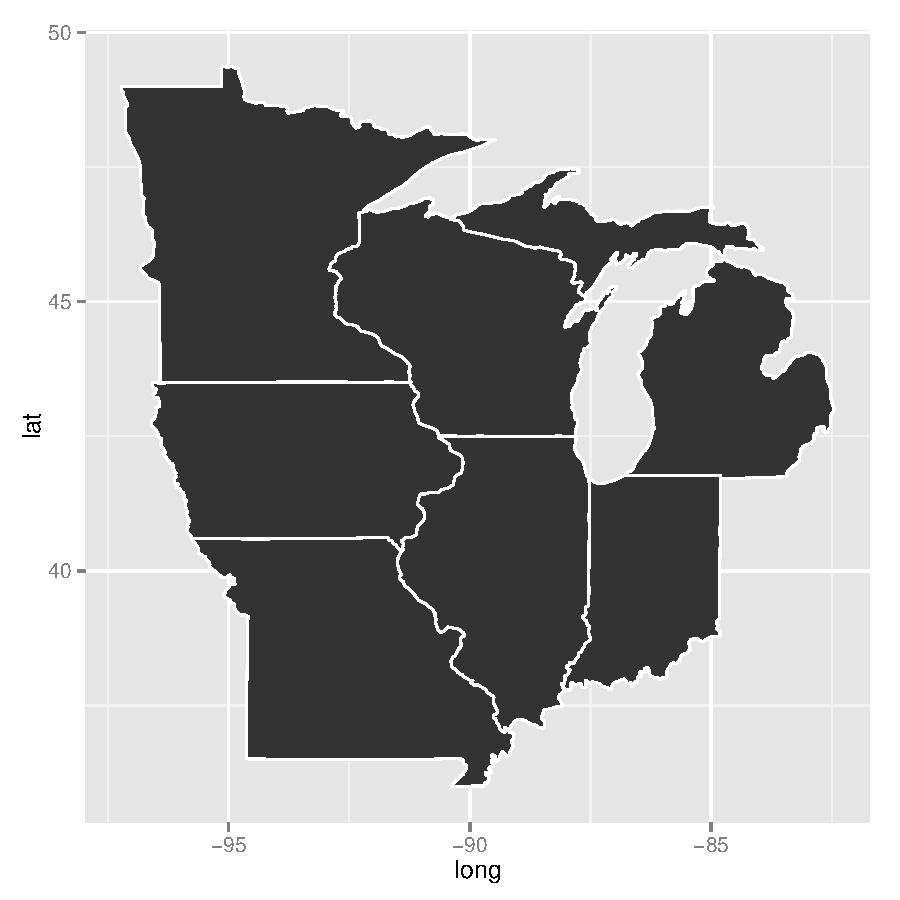
\includegraphics[height=6cm]{./plots/some-states.pdf}
\end{center}
\end{frame}
\begin{frame}[label=sec-15]{A hobby project}
\begin{itemize}
\item Internal talks at 3M typically given live to US audience; recorded for int'l
\item Organized two "reverse talks" to reach a wider global audience
\item Attendance records shattered
\item Wanted to visualize impact/reach!
\end{itemize}
\end{frame}
\begin{frame}[label=sec-16]{The inspiration}
\begin{center}
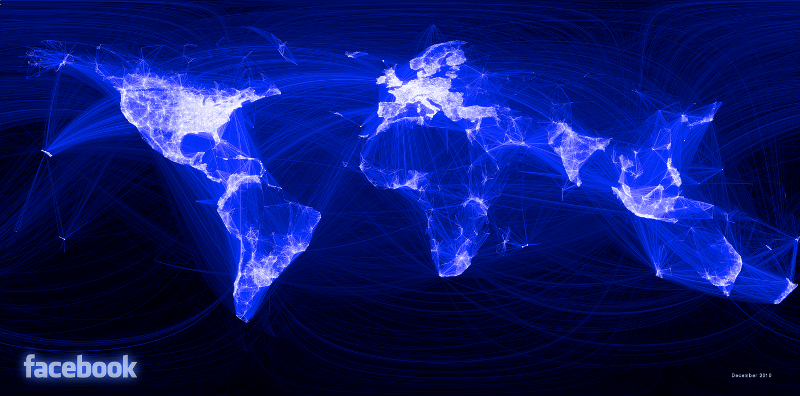
\includegraphics[height=6cm]{./img/facebook-map-lo.png}
\end{center}
\end{frame}
\begin{frame}[fragile,label=sec-17]{Calculating great circle arcs}
 \begin{itemize}
\item \texttt{gcIntermediate()} function from  \texttt{geosphere} package
\end{itemize}

\scriptsize
\begin{verbatim}
library(geosphere)
arc <- gcIntermediate(c(lon_1, lat_1), c(lon_2, lat_2),
                      n = steps, addStartEnd = T)
\end{verbatim}
\end{frame}
\begin{frame}[fragile,label=sec-18]{Crossing the Date Line}
 \scriptsize
\begin{verbatim}
# draw great circles from St. Paul to everywhere else
gcircles <- lapply(1:nrow(end), function(i) {                 # arc for each set
  temp <- gcIntermediate(start[, c("lon", "lat")],
                         end[i, c("lon", "lat")],
                         n = 50, addStartEnd = T,
                         breakAtDateLine = T)

  if(is.list(temp) == T) {                                    # were two half-paths returned?
    ids <- c(rep(paste0("i", i), nrow(temp[[1]])),            # if so, make id's for both halves
             rep(paste0("j", i), nrow(temp[[2]])))
    temp <- as.data.frame(rbind(temp[[1]], temp[[2]]))        # combine two sets of points
    temp$id <- ids                                            # assign ids for plotting
  }
  ...
\end{verbatim}
\normalsize
\end{frame}
\begin{frame}[fragile,label=sec-19]{The plot}
 \scriptsize
\begin{verbatim}
p <- ggplot()
p <- p + geom_polygon(aes(x = long, y = lat, group = group),               # world map
                      data = world, colour = "gray10", fill = "gray95")
p <- p + geom_line(aes(x = lon, y = lat, group = id),                      # great circles
                   dat = gcircles, lwd = 0.4, alpha = 0.5)
p <- p + geom_point(aes(x = lon, y = lat, size = sqrt(total/pi)),          # points
                    dat = talks_agg, colour = "#555599")
p <- p + scale_size("Total participants\n(both events)",                   # adjust legend
                    limits = c(0, max(sqrt(talks_agg$total / pi)) + 1),
                    breaks = sqrt(c(10, 50, 100) / pi),
                    labels = c(10, 50, 100), range = c(1, 10))
p <- p + theme_bw()                                                        # bw theme
p <- p + theme(axis.text = element_blank(), axis.title = element_blank(),  # tweak
               axis.ticks = element_blank(), panel.grid = element_blank(),
               legend.position = c(0.092, 0.15))
\end{verbatim}
\normalsize
\end{frame}

\begin{frame}[label=sec-20]{The result}
\normalsize


\begin{center}
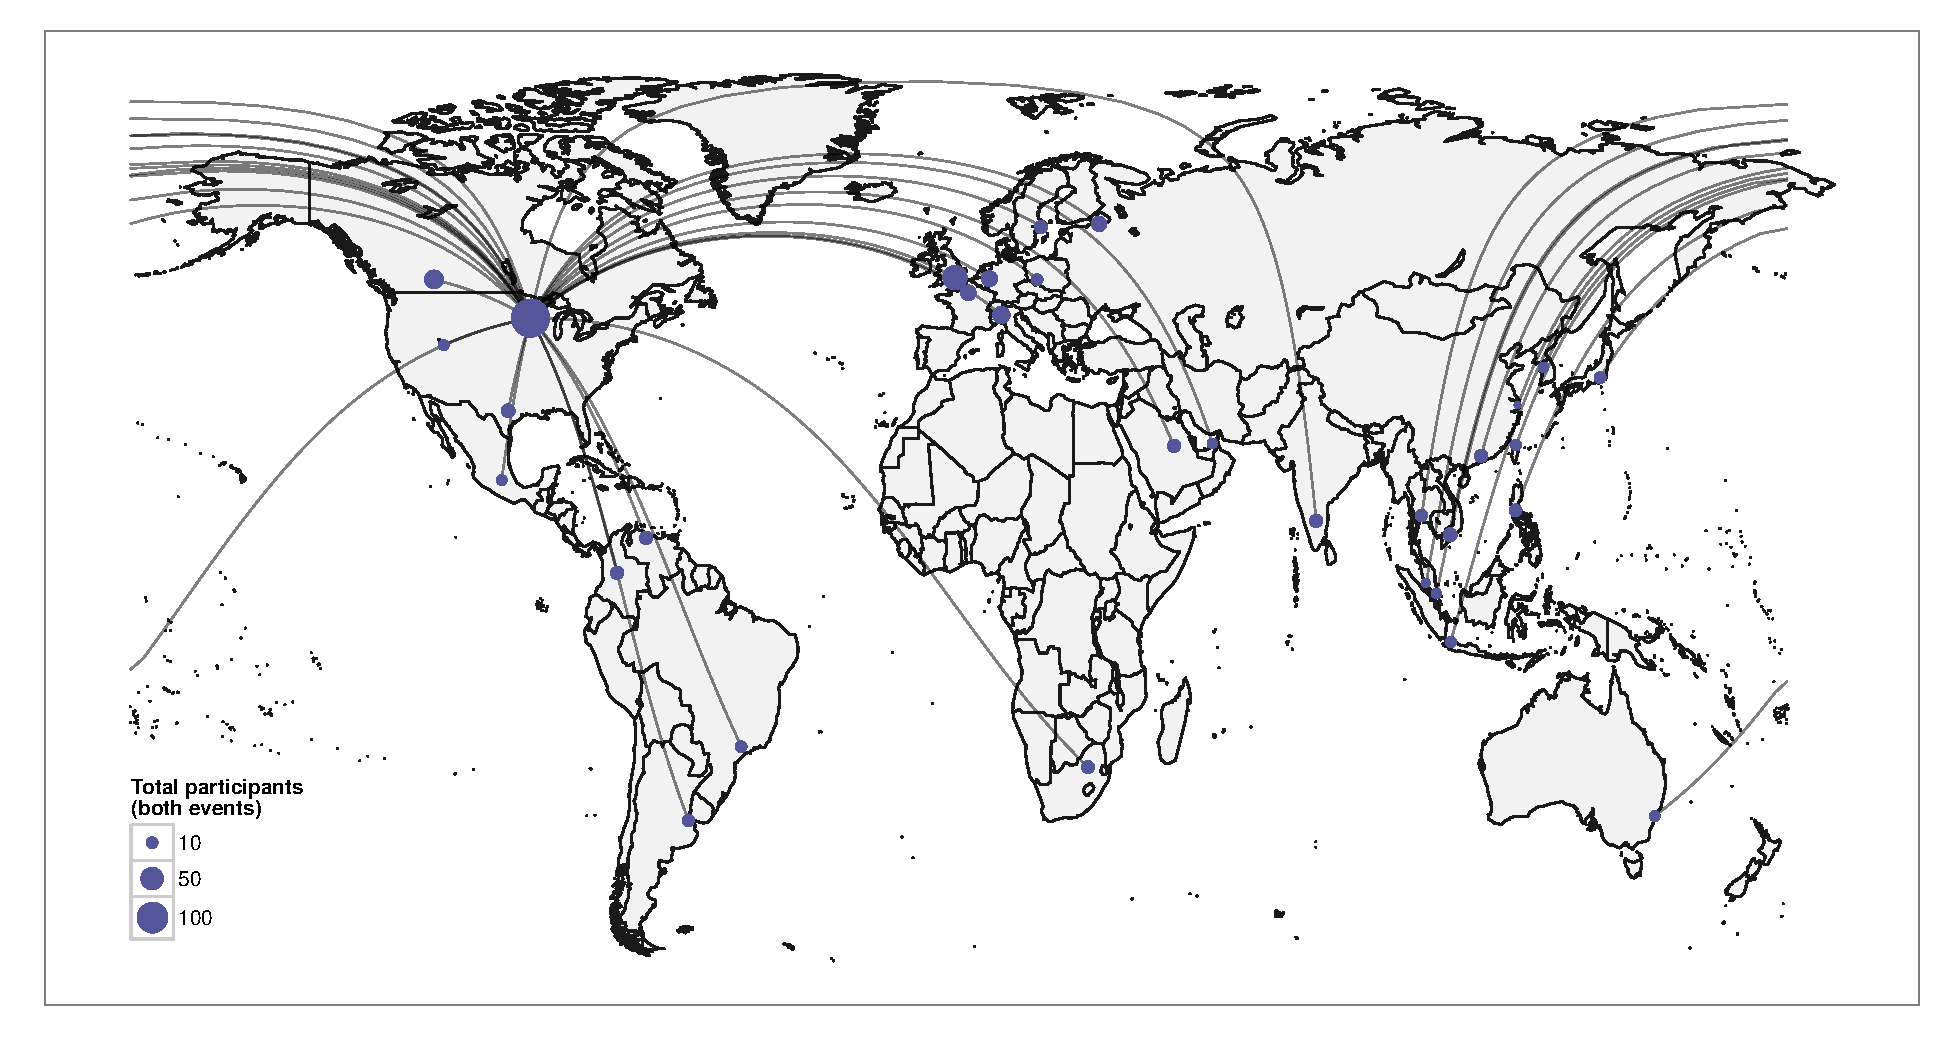
\includegraphics[height=6.5cm]{./plots/great-circles.pdf}
\end{center}
\end{frame}
\begin{frame}[label=sec-21]{Infographic}
\begin{center}
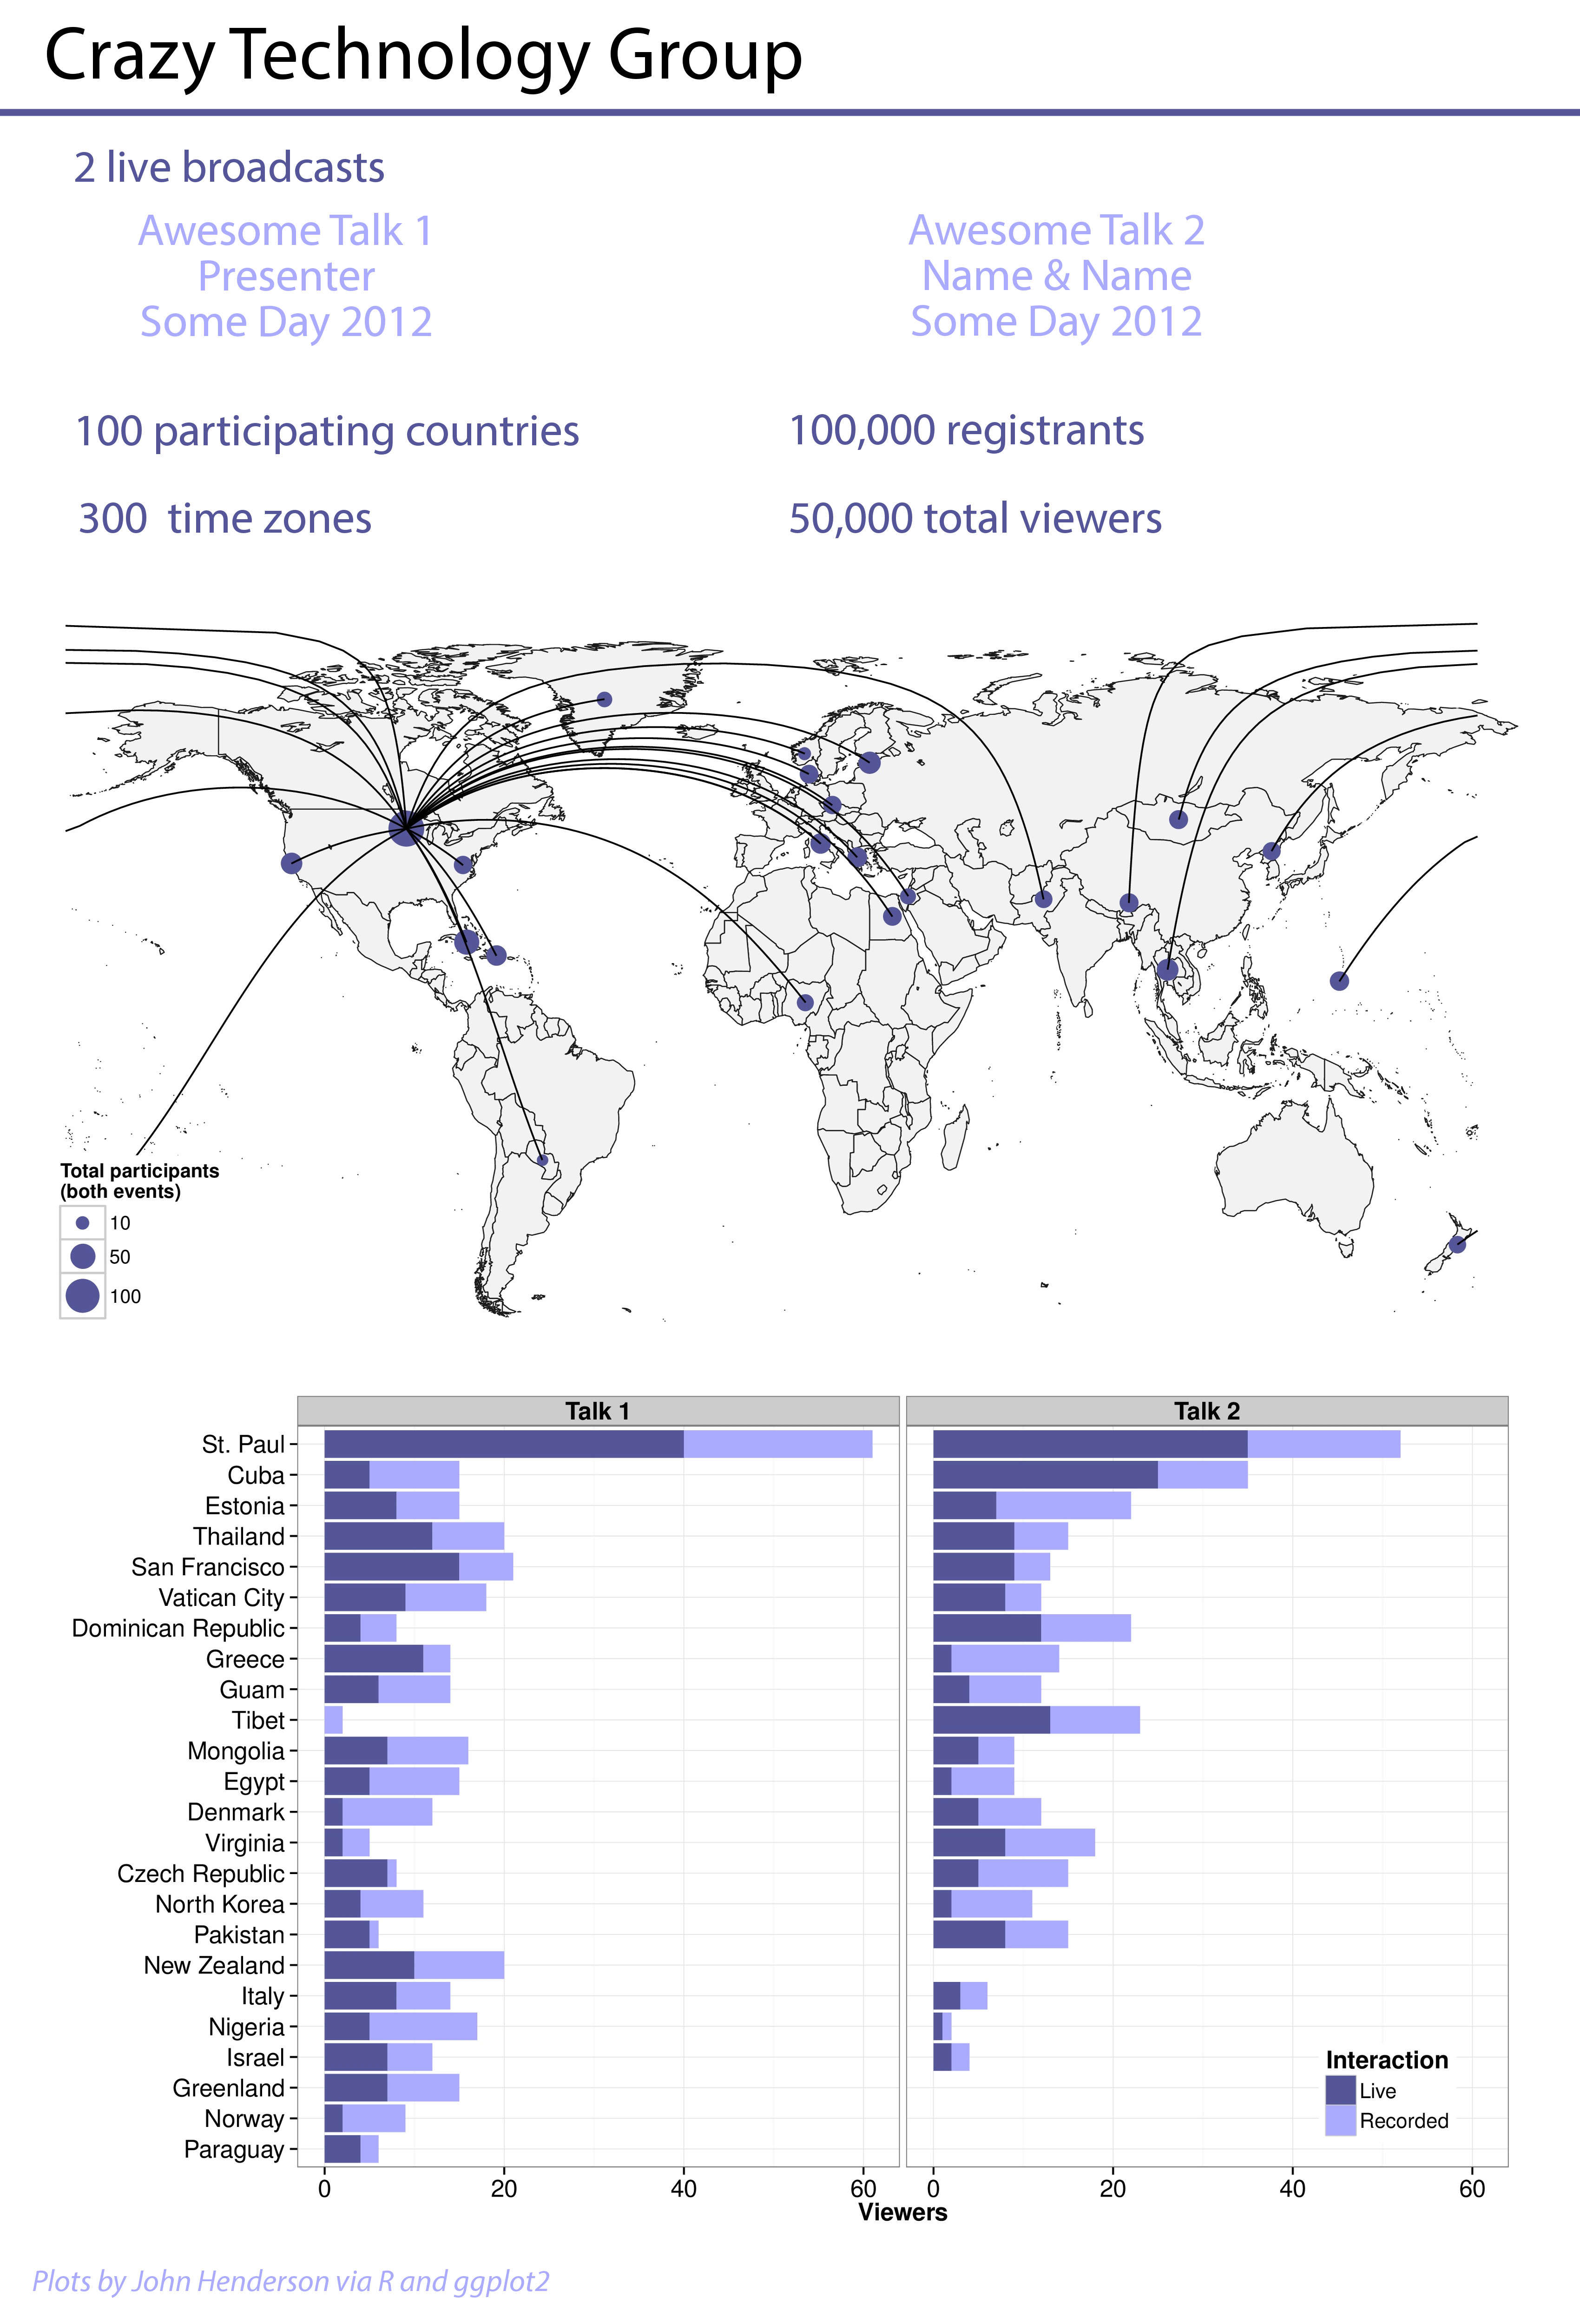
\includegraphics[height=6.5cm]{./img/infographic-flattened-lo.jpg}
\end{center}
\end{frame}
\begin{frame}[fragile,label=sec-22]{Creating \texttt{.kml} files for Google Earth}
 \begin{itemize}
\item Pretty easy! (Follow along with \href{http://www.nceas.ucsb.edu/scicomp/usecases/shapeFileToKML}{this}, \href{http://stackoverflow.com/questions/7813141/how-to-create-a-kml-file-using-r}{this}, \href{http://stackoverflow.com/questions/21487010/assistance-with-name-and-styleurl-in-kml-when-using-writeogr-from-rgdal}{this}, and \href{http://gsif.isric.org/doku.php?id=wiki:tutorial_plotkml}{this})
\end{itemize}

\scriptsize
\begin{verbatim}
talks_agg$size <- 100 * talks_agg$total

talks_sp <- talks_agg
coordinates(talks_sp) <- c("lon", "lat")                    # converts to spatial object
proj4string(talks_sp) <- CRS("+init=epsg:4238")             # G Earth coordinate system
talks_ll <- spTransform(talks_sp,
                        CRS("+proj=longlat +datum=WGS84"))  # Something else G Earth wants

# open a file connection and write the data with custom icon/size/label
kml_open("./data/talks-w-gcircles.kml")
kml_layer.SpatialPoints(talks_ll, colour = "white", labels = city, size = total,
                        shape="http://upload.wikimedia.org/wikipedia/commons/a/af/Tux.png")
kml_close("./data/talks-w-gcircles.kml")
\end{verbatim}
\normalsize
\end{frame}
\begin{frame}[fragile,label=sec-23]{Adding great circles}
 \begin{itemize}
\item A bit hackish, but manually writing the kml code works, too!
\end{itemize}

\scriptsize
\begin{verbatim}
# for each point set, generate the following kml syntax
gcircs <- lapply(1:nrow(end), function(i) {
  paste0("<Placemark><LineString><tesselate>1</tesselate><coordinates>",
         start$lon, ",", start$lat, " ", end[i, "lon"], ",", end[i, "lat"],
         "</coordinates></LineString></Placemark>") })

# combine the results into a single table
gcircs <- do.call(rbind, gcircs)

# print out each line of the above table
# retult can simply be pasted after last <Placemark> in .kml file
write.table(gcircs, row.names = F)
\end{verbatim}
\normalsize
\end{frame}
\begin{frame}[fragile,label=sec-24]{\texttt{.kml} file in Google Earth}
 \begin{center}
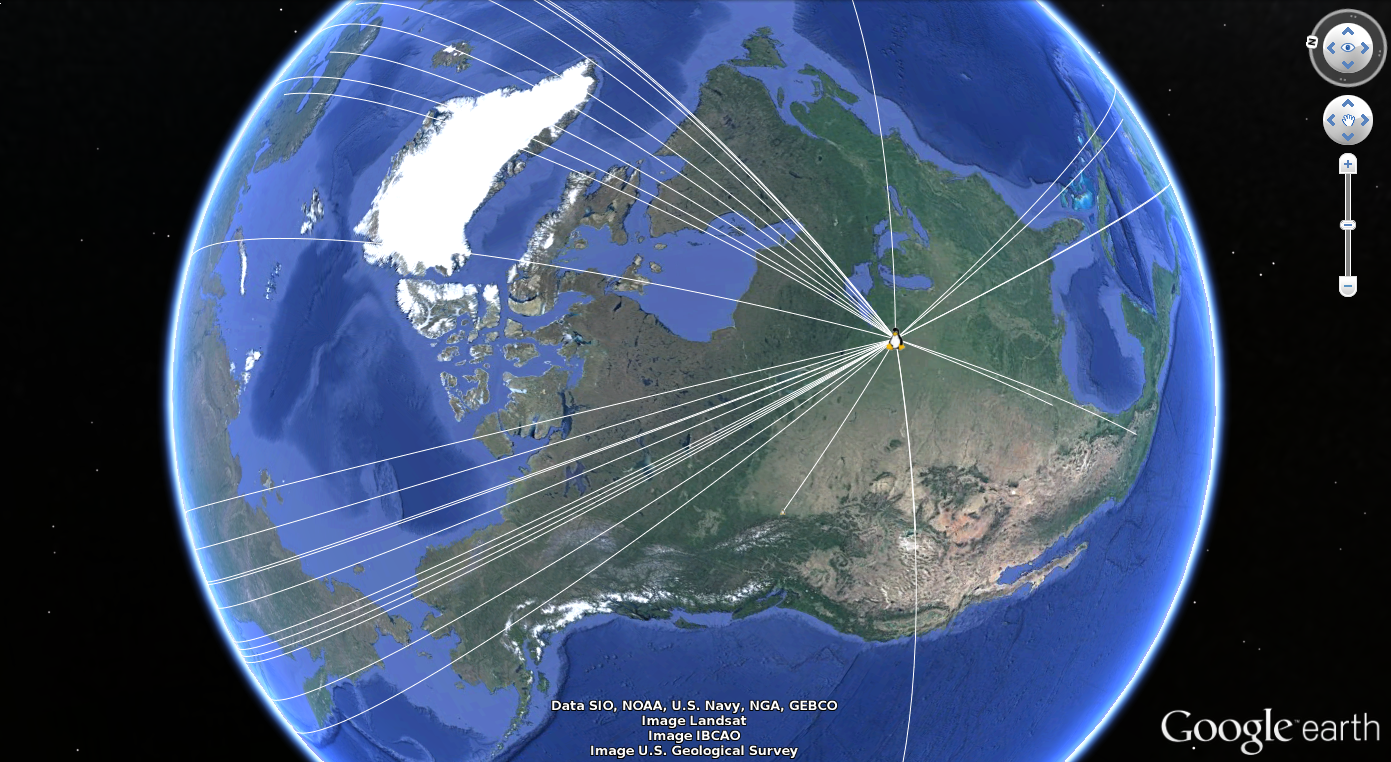
\includegraphics[height=6.5cm]{./img/talks-w-gcircles-kml.png}
\end{center}
\end{frame}
\begin{frame}[label=sec-25]{Getting some GPS data}
\begin{center}
\href{https://play.google.com/store/apps/details?id=com.fivasim.androsensor&hl=en}{\uline{AndroSensor}}
\end{center}

\begin{columns}
\begin{column}{0.45\textwidth}
\begin{center}
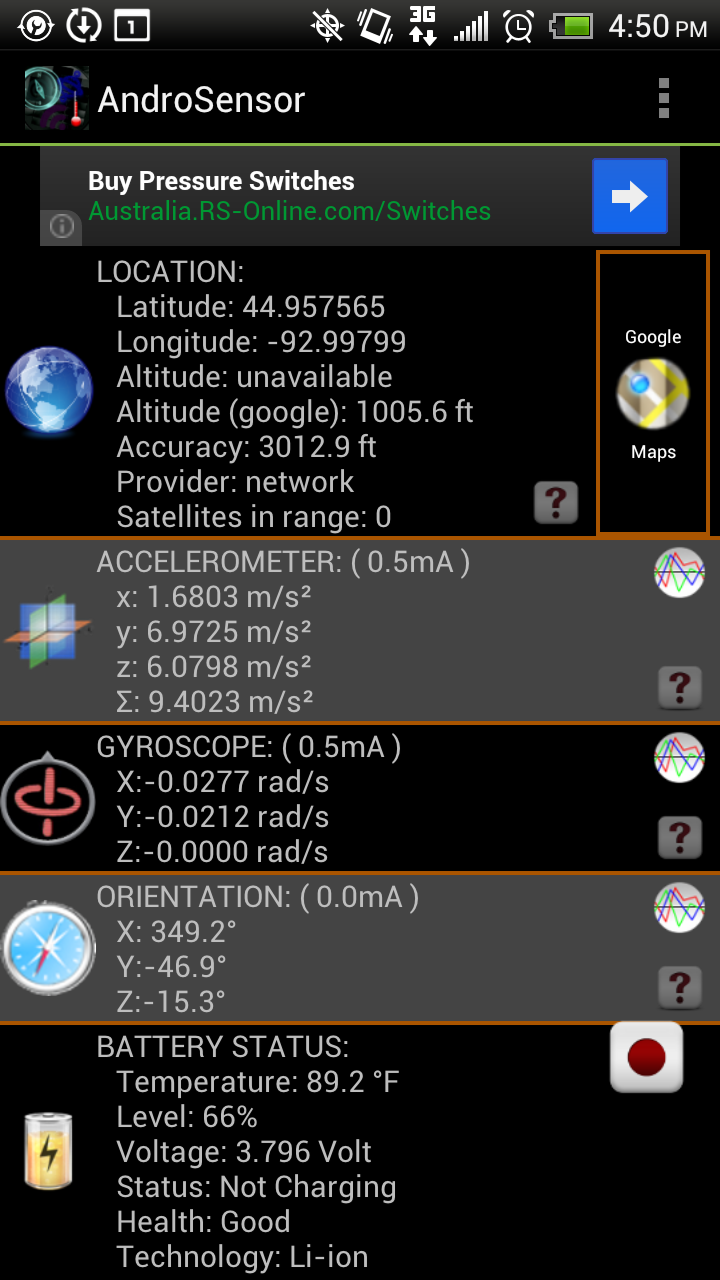
\includegraphics[height=5cm]{./img/andro-main.png}
\end{center}
\end{column}
\begin{column}{0.45\textwidth}
\begin{center}
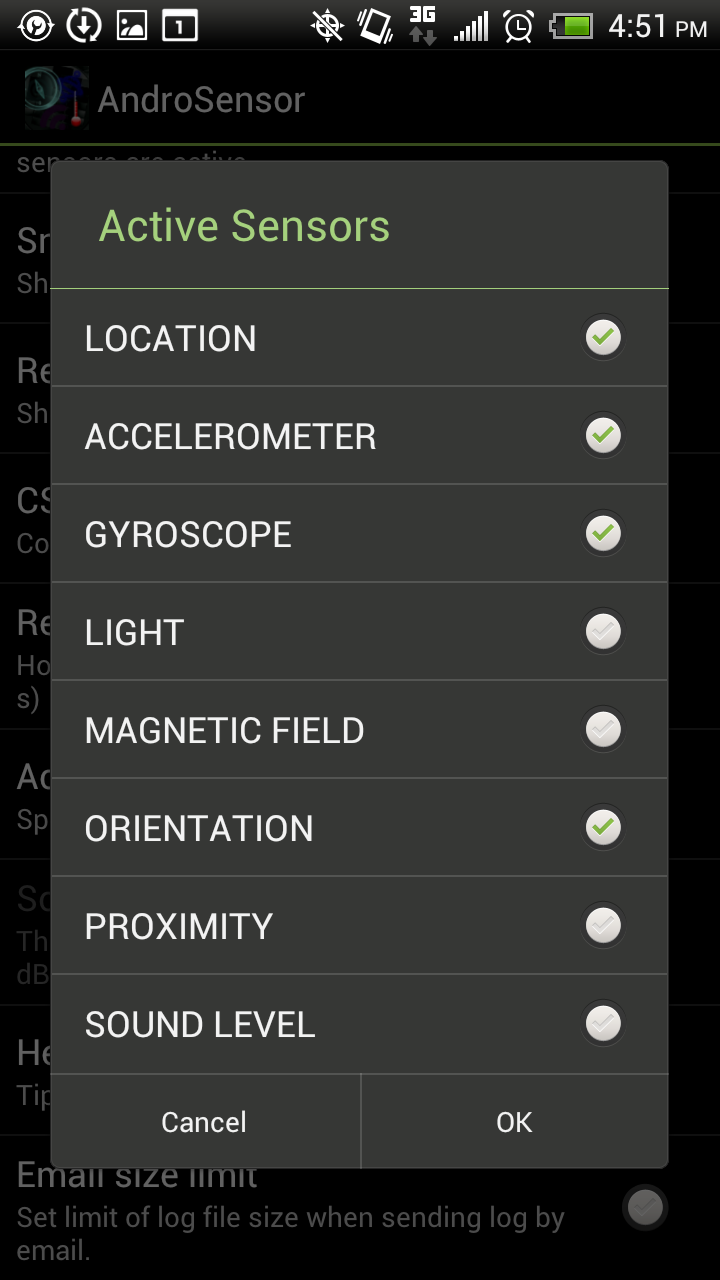
\includegraphics[height=5cm]{./img/andro-sensors.png}
\end{center}
\end{column}
\end{columns}
\end{frame}
\begin{frame}[fragile,label=sec-26]{Reading/cleaning the data}
 \scriptsize
\begin{verbatim}
gps <- read.csv("./data/gps-data.csv", sep = ";")

# subset to columns we're interested in
gps <- gps[, c(10, 11, 13, 18)]

# give the columns sensical names
names(gps) <- c("lat", "lon", "speed", "time")
head(gps, 5)
\end{verbatim}

\begin{verbatim}
       lat       lon speed time
1 44.92633 -93.09771    NA    5
2 44.92633 -93.09771    NA  505
3 44.92633 -93.09771    NA 1011
4 44.92633 -93.09771    NA 1532
5 44.92626 -93.09747     0 2032
\end{verbatim}

\normalsize
\end{frame}
\begin{frame}[fragile,label=sec-27]{Plot path and speed over a map}
 \scriptsize

\begin{verbatim}
p <- ggmap(gps_map)
p <- p + geom_point(aes(x = lon, y = lat, colour = speed), data = gps, size = 3)
p <- p + scale_colour_continuous(low = "black", high = "red", na.value = NA)
\end{verbatim}

\begin{center}
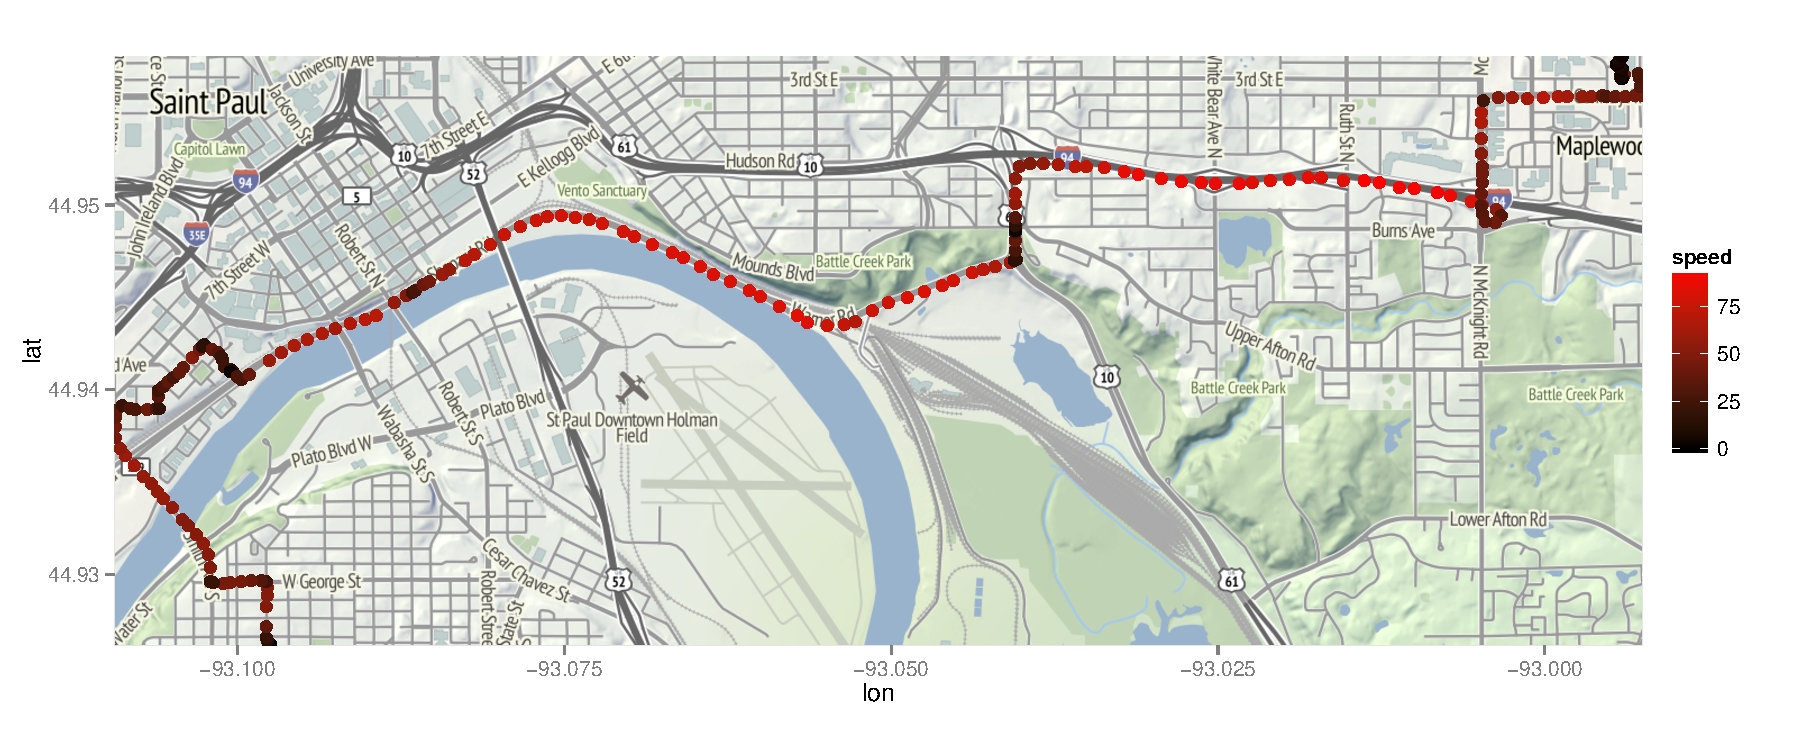
\includegraphics[height=5cm]{./plots/gps-map-over.pdf}
\end{center}

\normalsize
\end{frame}
\begin{frame}[fragile,label=sec-28]{Public transportation efficiency}
 \begin{itemize}
\item Background information can be found \href{https://github.com/tcrug/public-transpo}{here}
\end{itemize}

\scriptsize

\begin{verbatim}
transpo <- read.csv("./data/public-transpo.csv")

transpo_agg <- ddply(transpo, .(city, state), summarize,                    # stats by state
                     btus_pmile_ave = mean(btus_pmile),
                     density = mean(population) / mean(service_area_sq_mi))
transpo_agg$lookup <- paste0(transpo_agg$city, ", ", transpo_agg$state)

coords <- geocode(transpo_agg$lookup)                                       # city/state string

transpo_agg <- cbind(transpo_agg, coords)                                   # get lat/lon

# let's not run that again...
write.table(transpo_agg, file = "./data/transpo-agg-geocoded.csv", row.names = F, sep = ",")
\end{verbatim}
\normalsize
\end{frame}
\begin{frame}[fragile,label=sec-29]{Efficiency visualized}
 \scriptsize

\begin{verbatim}
plot <- read.csv("./data/transpo-agg-geocoded.csv")
plot <- plot[plot$state != "AK" & plot$state != "HI", ]
usa <- map_data("state")
plot <- plot[order(plot$btus_pmile_ave), ]
p <- ggplot() + geom_polygon(aes(x = long, y = lat, group = group),
                             data = usa, fill = "gray95", colour = "gray10")
p <- p + geom_point(aes(x = lon, y = lat, colour = btus_pmile_ave,
                    size = sqrt(density)/pi), data = plot)
p <- p + scale_colour_gradient("BTUs / passenger-mile", trans = "log")
p <- p + scale_x_continuous("") + scale_y_continuous("")
p <- p + scale_size_continuous("Passengers / Sq. Mile", breaks = c(10, 20, 30, 40),
                               labels = round((c(10, 20, 30, 40)*pi)^2, 0),
                               range = c(1, 8))
p <- p + theme_bw() + theme(axis.text = element_blank(), axis.ticks = element_blank())
\end{verbatim}

\normalsize
\end{frame}
\begin{frame}[label=sec-30]{Efficiency visualized}
\begin{center}
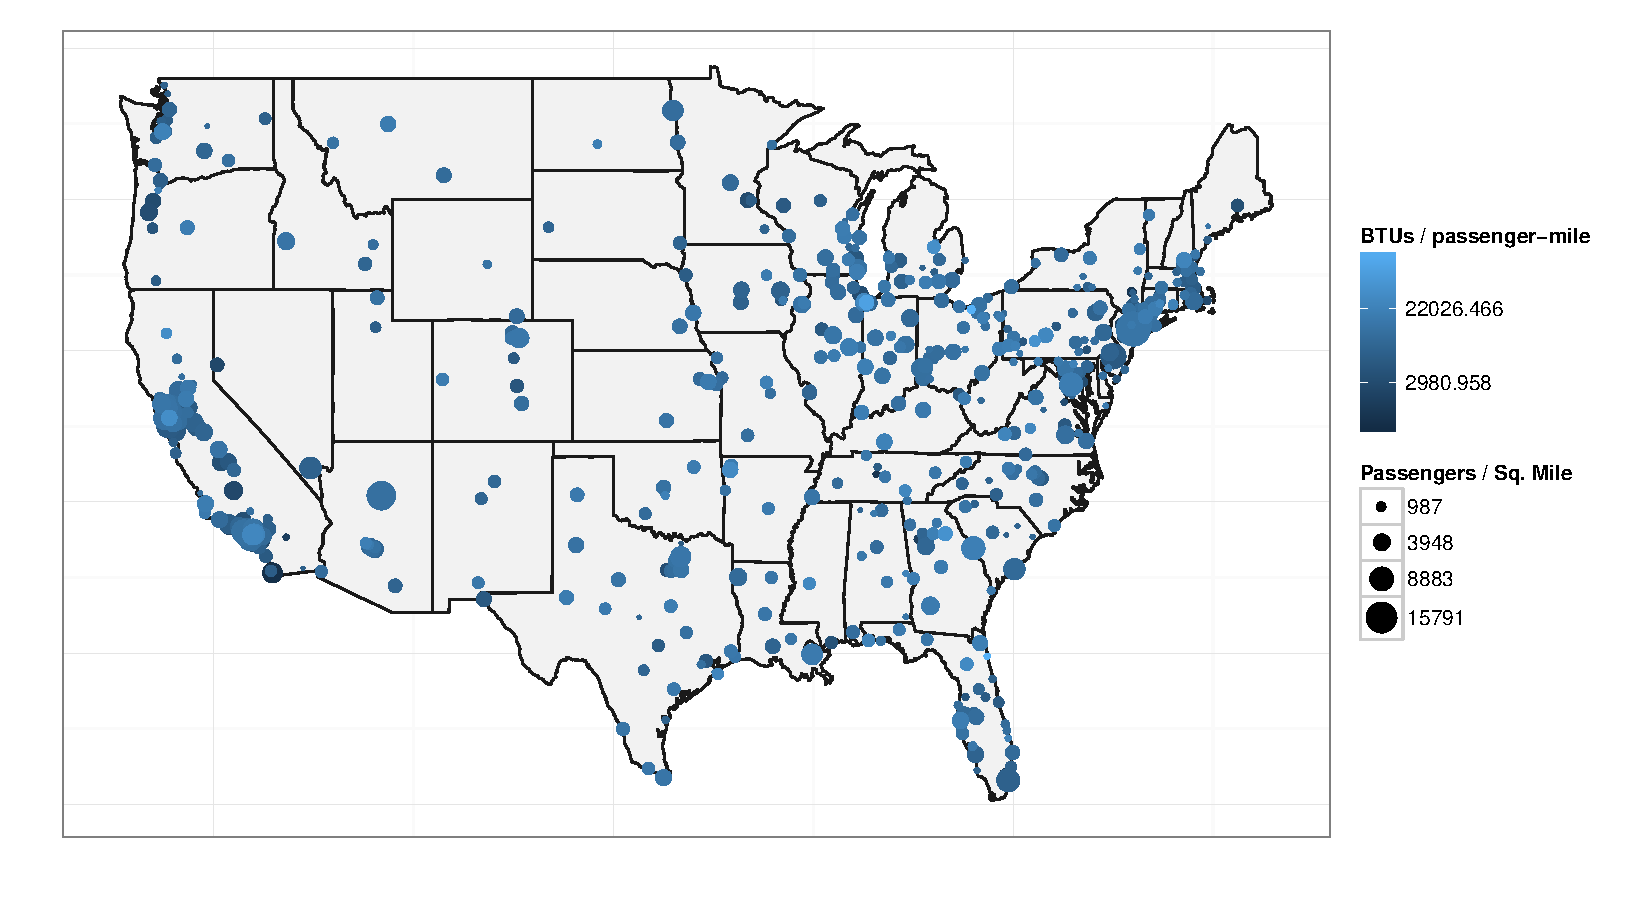
\includegraphics[height=6.5cm]{./plots/transpo-plot.pdf}
\end{center}

\normalsize
\end{frame}
\begin{frame}[fragile,label=sec-31]{Converting data to \texttt{.json} for d3}
 \begin{itemize}
\item R is an excellent for working with data
\begin{itemize}
\item Reshape (wide \(\leftrightarrow\) long)
\item Calculate columns
\item Summarize, e.g. with \texttt{ddply}
\end{itemize}
\item Manipulate in R, then output to \texttt{.json}, d3's friend
\item Helpful function found \href{http://theweiluo.wordpress.com/2011/09/30/r-to-json-for-d3-js-and-protovis/}{here}, \texttt{toJSONarray()}
\end{itemize}

\scriptsize
\begin{verbatim}
plot_json <- toJSONarray(plot)         # function defined in link above
file_con <- file("./d3/transpo.json")  # create file
writeLines(plot_json, file_con)        # write results to file
close(file_con)
\end{verbatim}
\normalsize
\end{frame}

\begin{frame}[label=sec-32]{And voila, a d3 version!}
\begin{center}
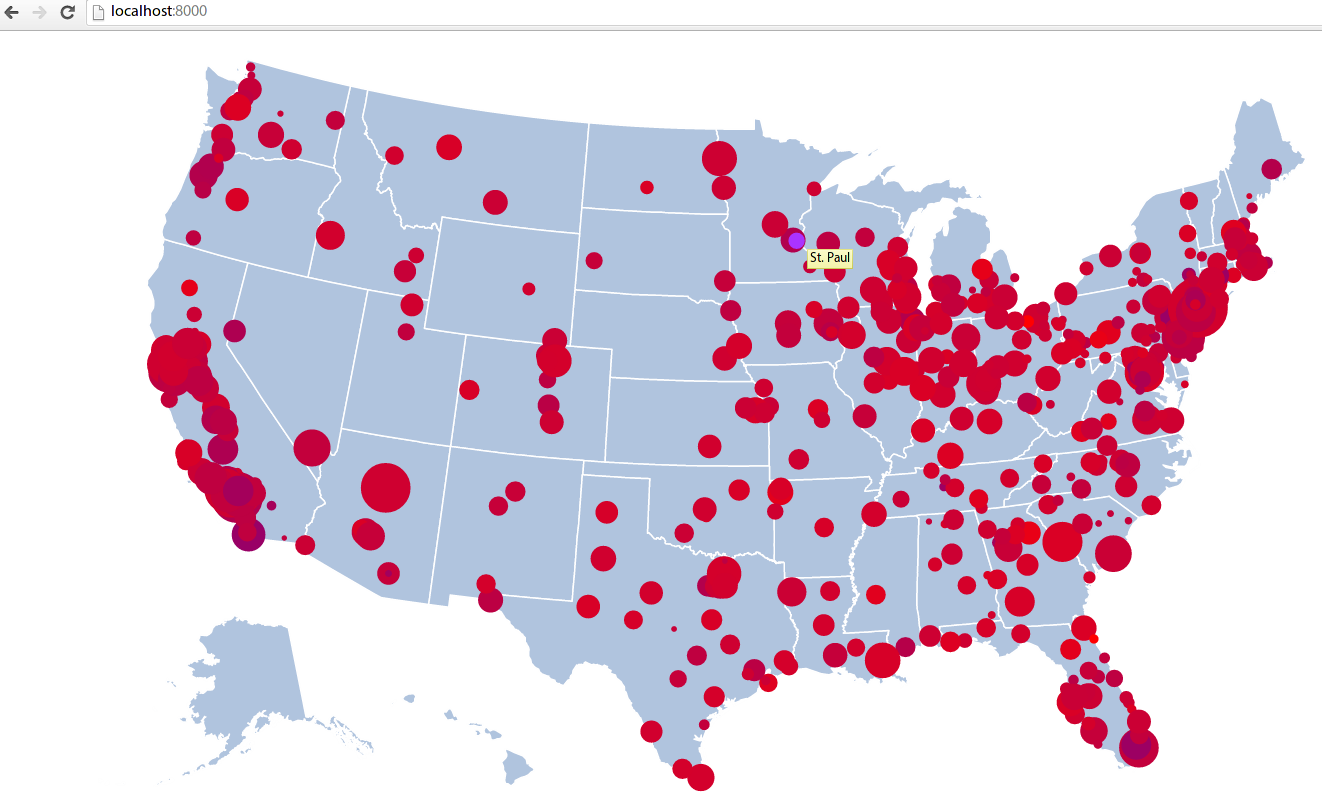
\includegraphics[height=6.5cm]{./img/transpo-d3.png}
\end{center}
\end{frame}
\begin{frame}[fragile,label=sec-33]{Visualizing work activity}
 \begin{itemize}
\item Tracked work projects with \href{https://play.google.com/store/apps/details?id=com.rauscha.apps.timesheet}{Timesheet} (projects, tags, location)
\end{itemize}

\scriptsize
\begin{verbatim}
time <- read.csv("./data/timesheet.csv")              # read data
time <- time[!is.na(time$Location), ]                 # remove entries w/ no loc
mmm_box <- c(left = -93.0053, bottom = 44.9485,       # bounding box
             right = -92.9844, top = 44.9632)
mmm <- get_map(location = mmm_box, source = "stamen", # get map
               maptype = "toner", crop = T)

time <- ddply(time, .(Location), summarize,           # total time per loc
              total = sum(Duration)) 

# figure out building coords and merge with timesheet data
bldgs <- data.frame(loc = time$Location))
bldgs$lat <-  c(44.9515, 44.9576, 44.9525, 44.9545, 44.9577, 44.955,  44.9512, 44.9619, 44.9585)
bldgs$lon <- -c(93.0033, 92.9935, 92.9955, 92.9982, 92.9998, 92.9897, 93.0009, 93.00,   92.9942)
time <- merge(time, bldgs, by.x = "Location", by.y = "loc")

# line from my main building to each of the other ones
lines <- data.frame(lat = c(rep(bldgs[2, "lat"], 8), bldgs[c(1, 3:9), "lat"]),
                    lon = c(rep(bldgs[2, "lon"], 8), bldgs[c(1, 3:9), "lon"]),
                    grp = rep(1:8, 2))

p <- ggmap(mmm)
p <- p + geom_line(aes(x = lon, y = lat, group = grp),
                   data = lines, colour = "steelblue")
p <- p + geom_point(aes(x = lon, y = lat, size = sqrt(total)/pi),
                    data = time, fill = "steelblue", colour = "black", pch = 21)
p <- p + scale_x_continuous("") + scale_y_continuous("")
p <- p + scale_size_continuous("Hours", breaks = c(0.5, 1, 1.5, 2),
                               labels = c(2.5, 10, 20, 40), range = c(2, 6))
p <- p + theme_bw() + theme(axis.text = element_blank(), axis.ticks = element_blank())
p
\end{verbatim}
\normalsize
\end{frame}
\begin{frame}[label=sec-34]{Visualizing work activity}
\begin{center}
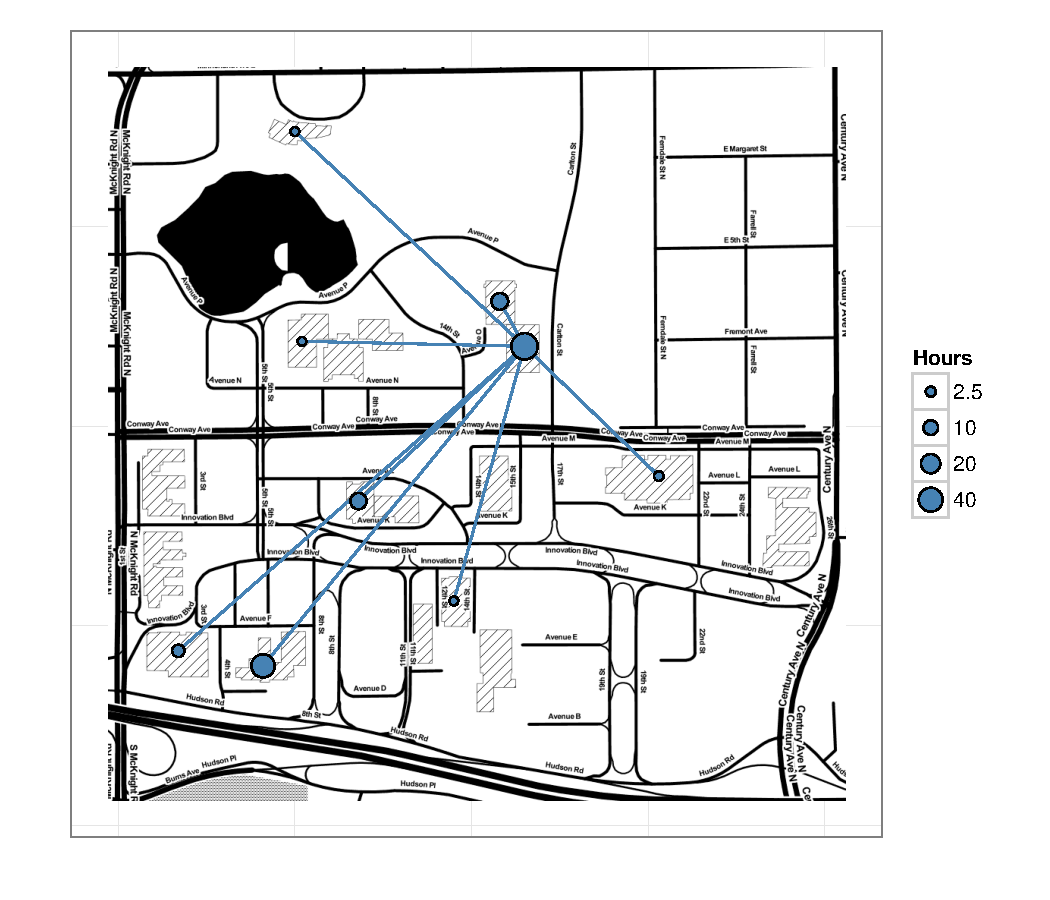
\includegraphics[height=6.5cm]{./plots/mmm-timesheet.pdf}
\end{center}
\end{frame}
\begin{frame}[fragile,label=sec-35]{\texttt{R} packages used}
 \begin{itemize}
\item Getting coordinates/working with Google: \texttt{ggmap}
\item Great circle paths: \texttt{geosphere}
\item Larger scale maps: \texttt{maps}
\item Projection conversion/KML output: \texttt{rgdal}, \texttt{maptools}, \texttt{sp}, and \texttt{plotKML}
\item Summary computations on data: \texttt{ddply()} function from \texttt{plyr}
\item Reshaping data (wide \(\leftrightarrow\) long): \texttt{reshape2}
\item Plotting: \texttt{ggplot2}
\end{itemize}
\end{frame}
\begin{frame}[fragile,label=sec-36]{References}
 \begin{itemize}
\item \href{http://stat405.had.co.nz/ggmap.pdf}{ggmap: Spatial Visualization with ggplot2}, Kahle \& Wickham
\item \href{http://uchicagoconsulting.wordpress.com/2011/04/18/how-to-draw-good-looking-maps-in-r/}{How to draw good looking maps in R}, uchicagoconsulting
\item \href{http://www.stanford.edu/~cengel/cgi-bin/anthrospace/great-circles-on-a-recentered-worldmap-in-ggplot}{Great circles on a recentered worldmap}, AnthroSpace
\item \href{http://flowingdata.com/2011/05/11/how-to-map-connections-with-great-circles/}{How to map connections with great circles}, FlowingData
\item \href{http://stackoverflow.com/questions/21487010/assistance-with-name-and-styleurl-in-kml-when-using-writeogr-from-rgdal}{SO question on creating \texttt{.kml} files}
\item For any given package, find the documentation on \href{http://cran.r-project.org/}{CRAN}
\end{itemize}

\vspace{0.5cm}

Code and files from this presentation are on \href{https://github.com/jwhendy/devFest-geo}{github}!
\end{frame}
\begin{frame}[label=sec-37]{Tools}
Presentation made entirely with open source software!

\begin{center}
\begin{center}
\begin{tabular}{llll}

\includegraphics[height=1.5cm]{./img/emacs.png} & 
\includegraphics[height=1.5cm]{./img/org-mode.png} & 
\includegraphics[height=1.5cm]{./img/r.png} & 
\includegraphics[height=1.5cm]{./img/arch.png}\\
\end{tabular}
\end{center}
\end{center}

\begin{itemize}
\item \href{http://www.gnu.org/software/emacs/}{Emacs} and \href{http://orgmode.org/}{Org-mode} for reproducible code environment
\item \href{http://www.latex-project.org/}{\LaTeX} / \href{http://www.ctan.org/tex-archive/macros/latex/contrib/beamer/}{Beamer} for typesetting
\item \href{http://blog.barisione.org/2007-09/torino-a-pretty-theme-for-latex-beamer/}{Torino} Beamer theme so that it wasn't obvious I was using Beamer
\end{itemize}
\end{frame}
% Emacs 24.3.1 (Org mode 8.2.5h)
\end{document}
